
\appendix 
\section{Appendix Figures}
\renewcommand{\thefigure}{A\arabic{figure}}
\setcounter{figure}{0}

\begin{figure}[!h]
    \centering 
    \caption{Average non-zero tax paid by Chinese immigrants to Canada, by year of arrival in Canada, as recorded by the Chinese Register, which tracked all Chinese immigrants who entered Canada and/or paid the Head Tax between 1885 and 1949 \citep{chineseregister}. Note that among Chinese immigrants who arrived in Canada prior to 1885, only those who re-entered Canada at some point following 1885 were forced to pay the Head Tax and therefore recorded in the registry, which is why we observe non-zero payments among immigrants arriving prior to 1885.}
    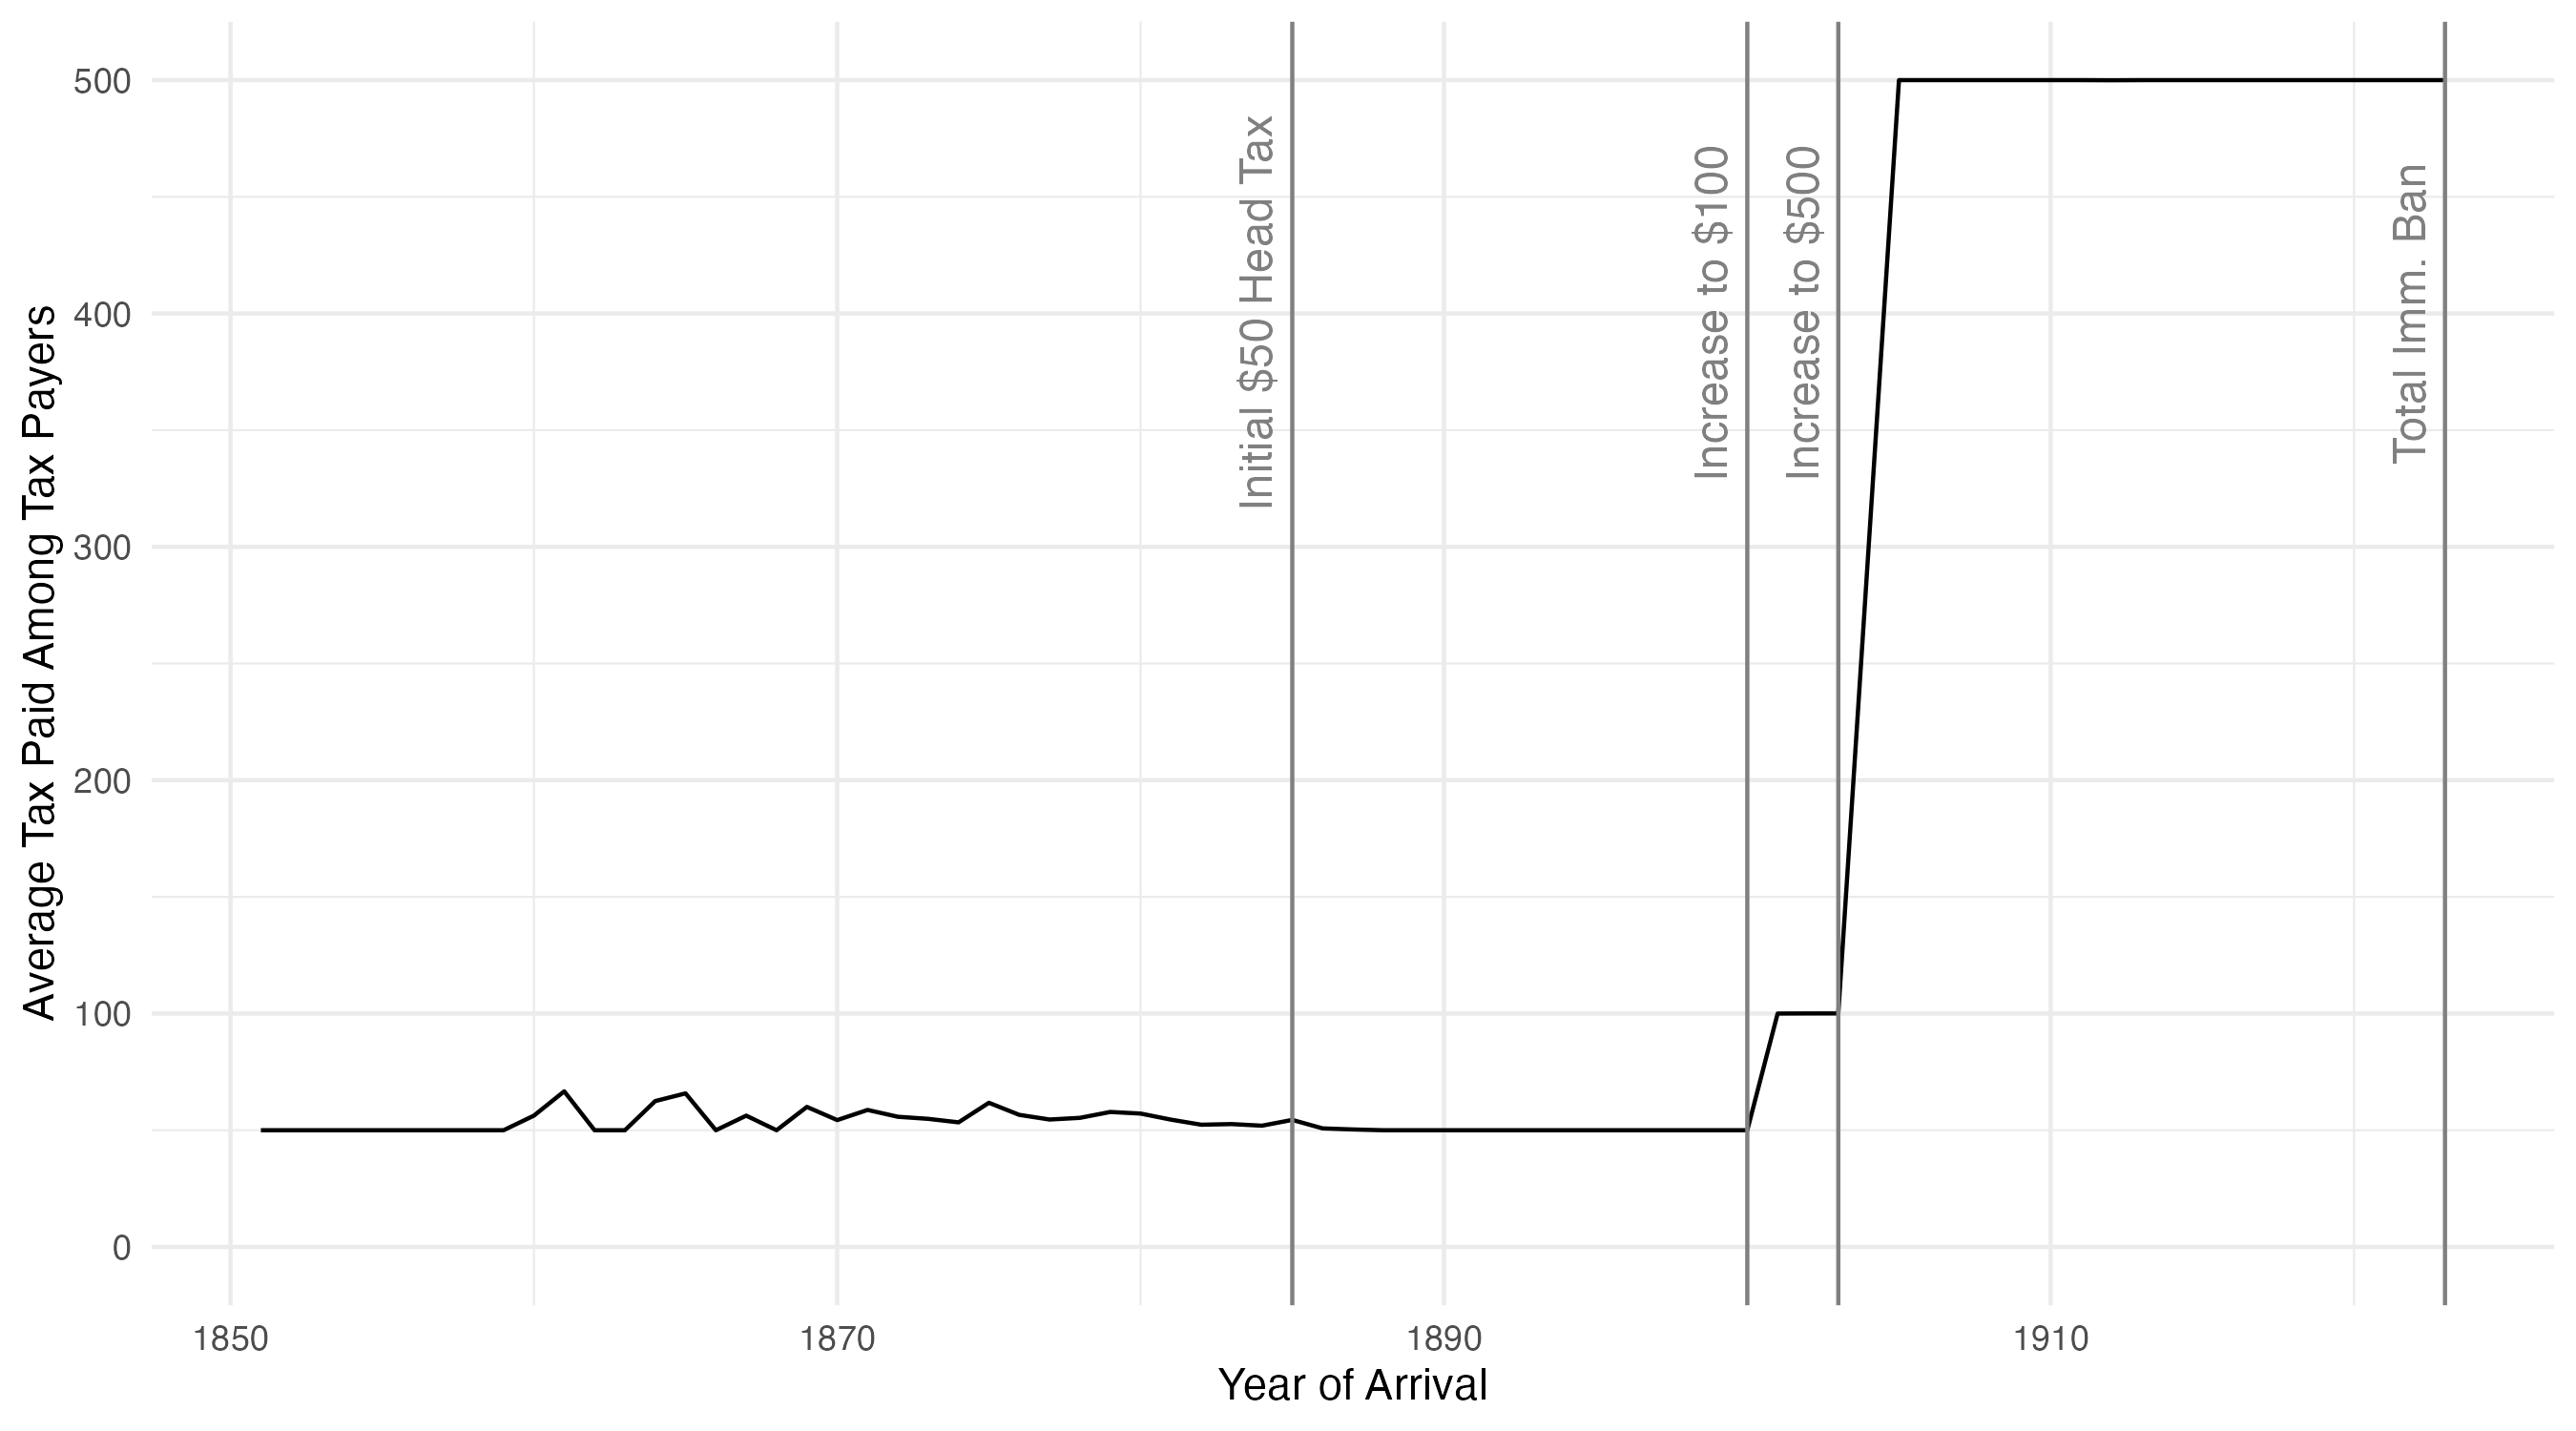
\includegraphics[width=\textwidth]{../../figs/fig1_taxespaid.png}
    \label{fig:taxpaid}
\end{figure}
\newpage 

% \begin{figure}
%     \centering 
%     \caption{census data -- chi/all imm inflows}
%     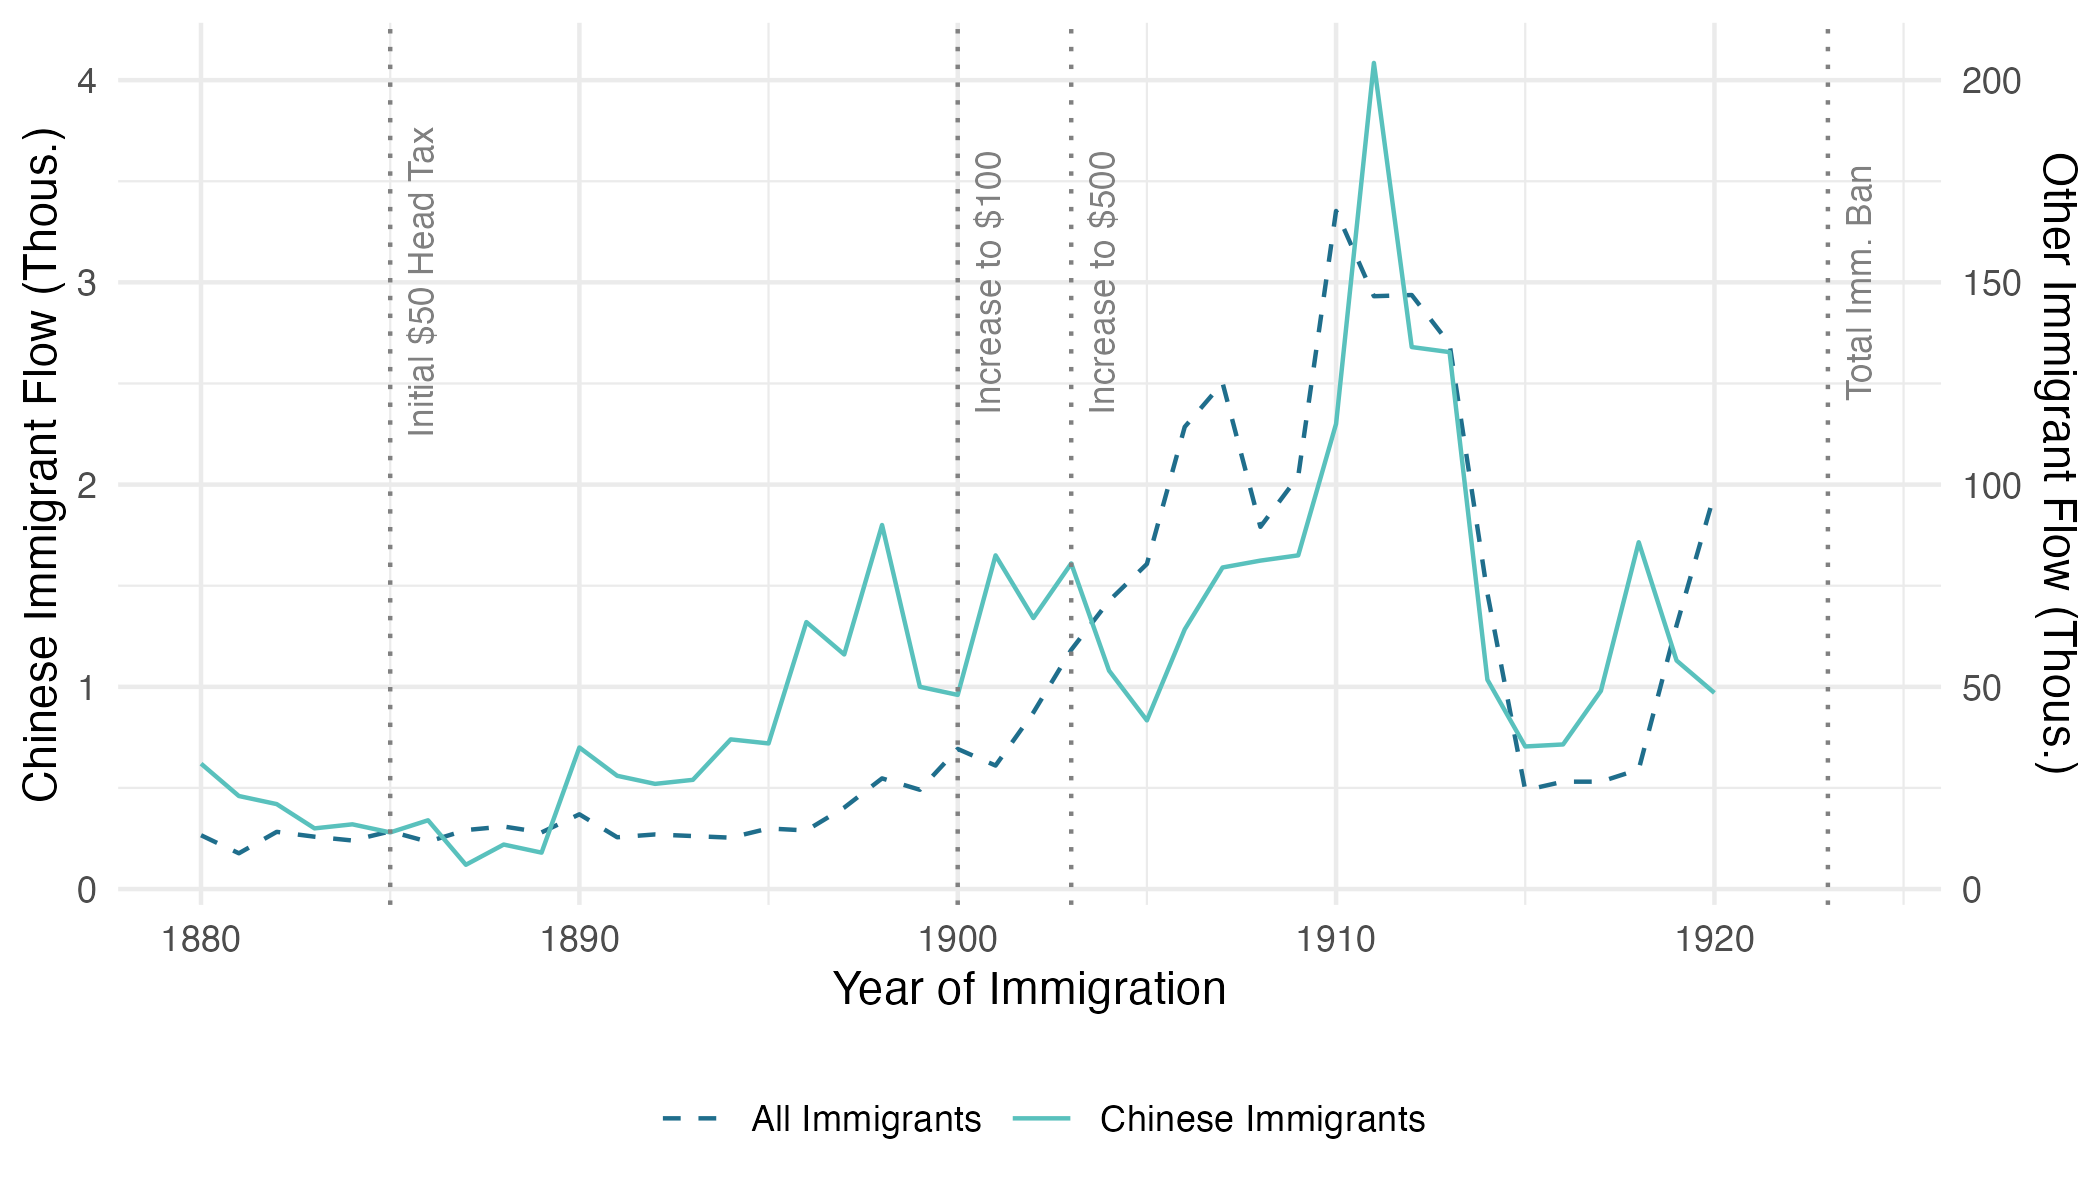
\includegraphics[width=\textwidth]{../../figs/fig2_census_flow.png}
%     \label{fig:immflowcensus}
% \end{figure}


% \begin{figure}
%     \centering 
%     \caption{asdf}
%     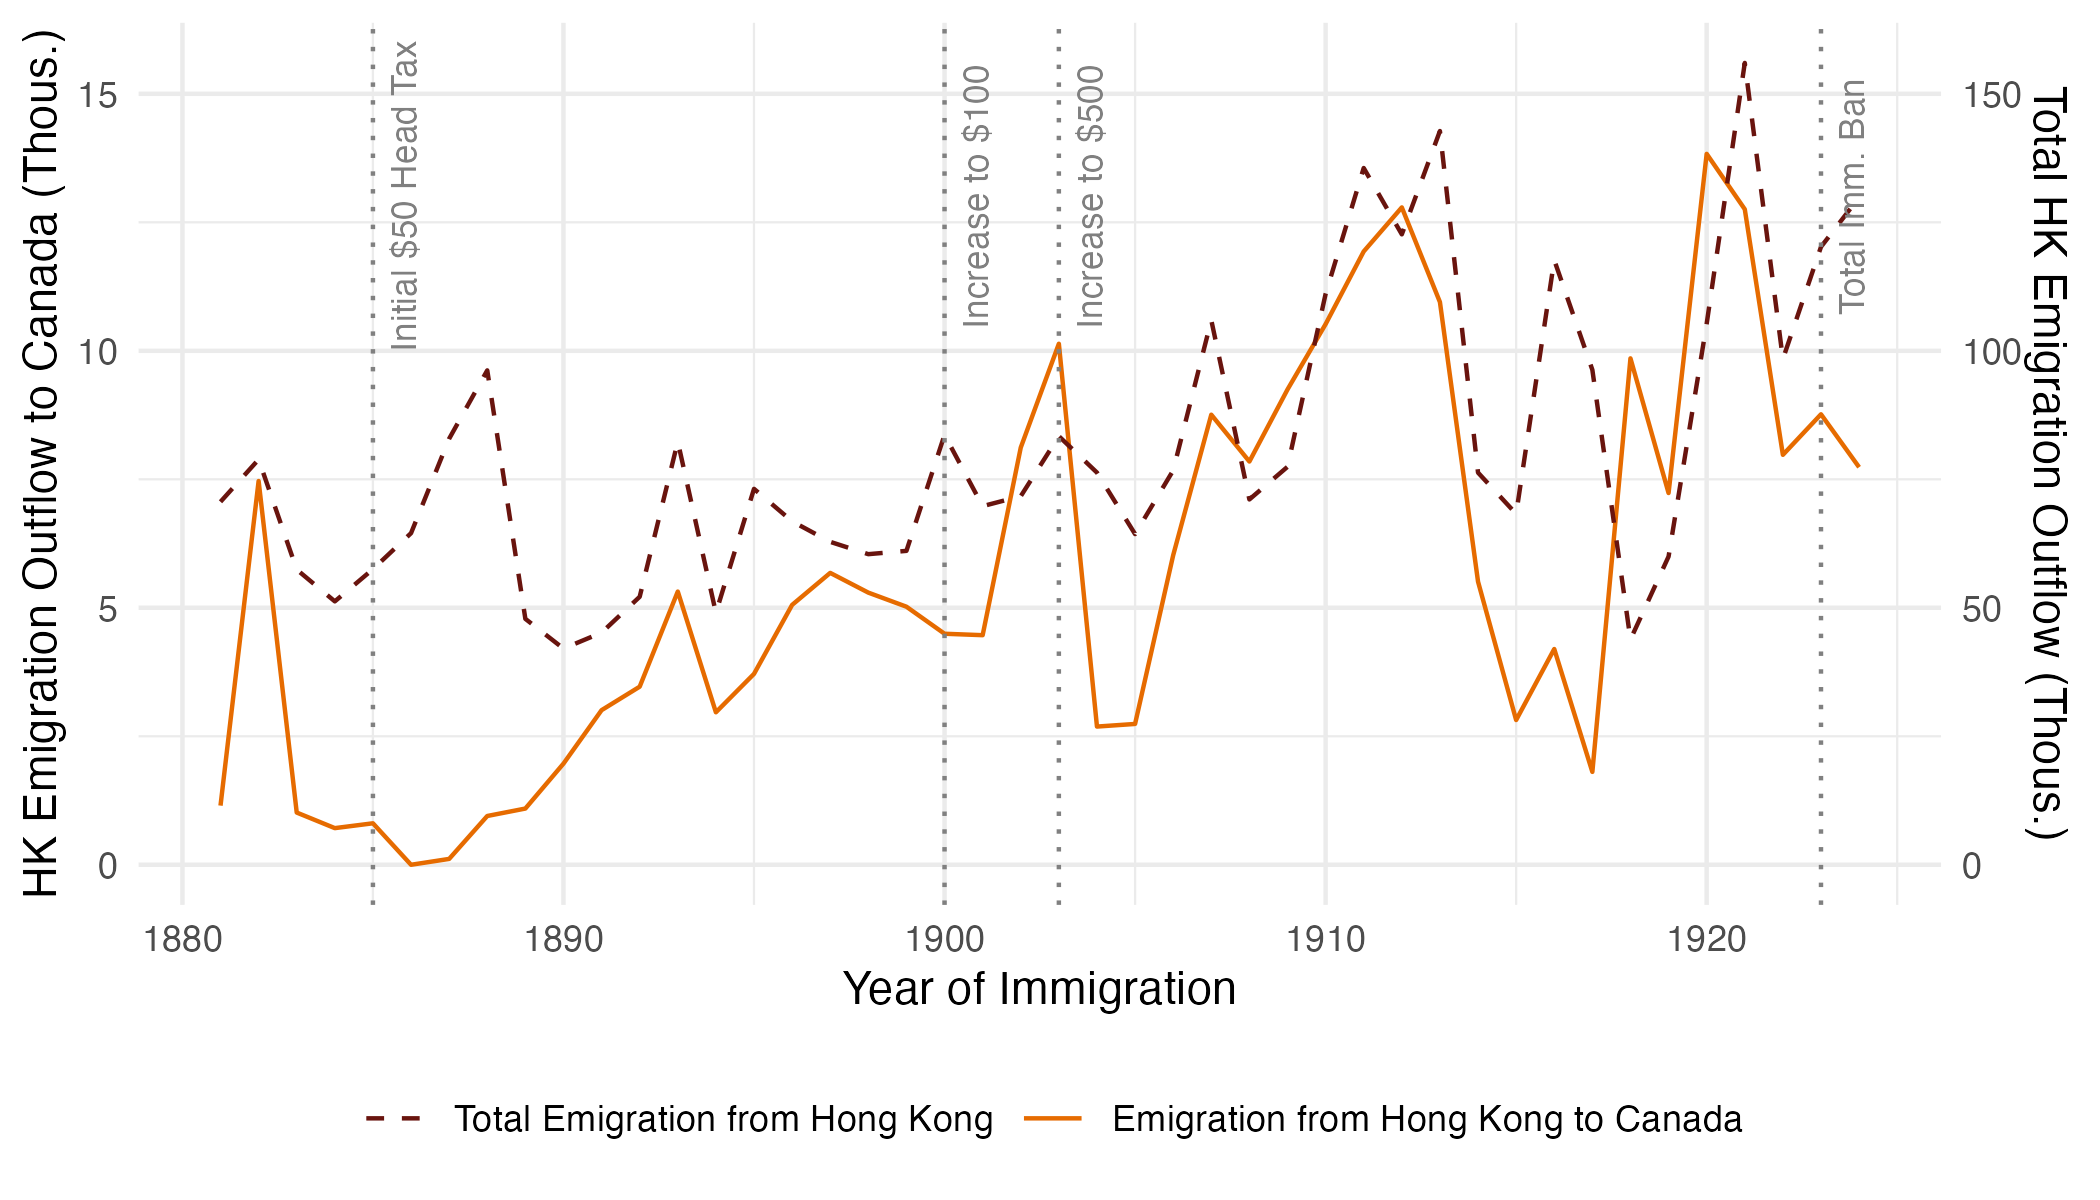
\includegraphics[width=\textwidth]{../../figs/fig2_flow_hkemig.png}
%     \label{fig:hkemig}
% \end{figure}

% \begin{figure}
%     \centering 
%     \caption{asdf}
%     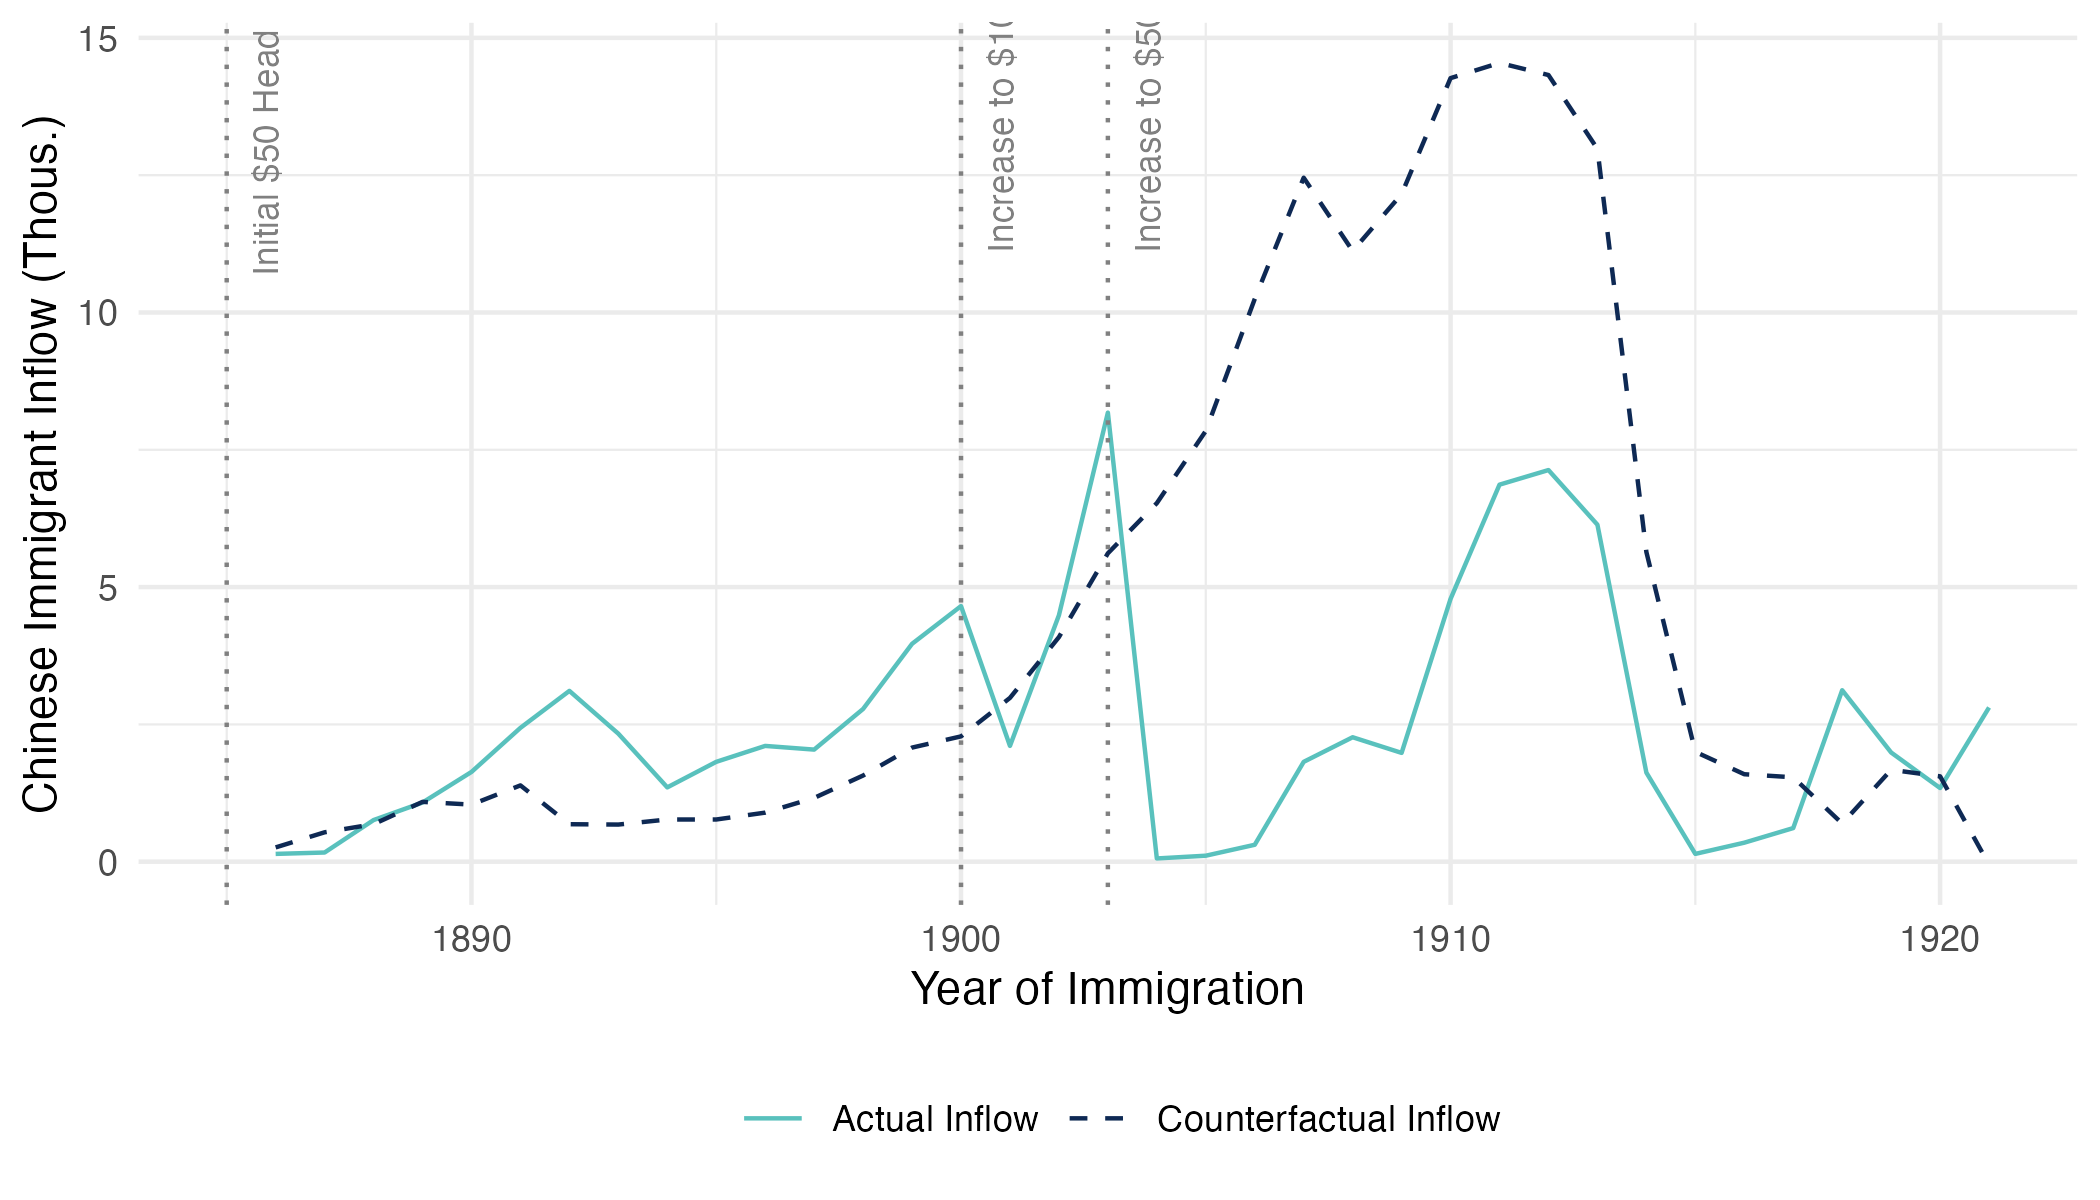
\includegraphics[width=\textwidth]{../../figs/immflow_counterfactual.png}
%     \label{fig:immflowcf}
% \end{figure}

\section{Comparison of Chinese Immigration and Hong Kong Emigration Data}
\begin{figure}[!h]
    \centering 
    \caption{Inflow of Chinese immigrants to Canada (solid blue line) as measured by the Chinese Register \citep{chineseregister} and outflow of emigrants from Hong Kong to Canada (dotted orange line) as measured by the Hong Kong Harbourmaster reports \citep{hkharbourmaster}. Vertical dotted lines mark years in which the Head Tax was initially created or increased.}
    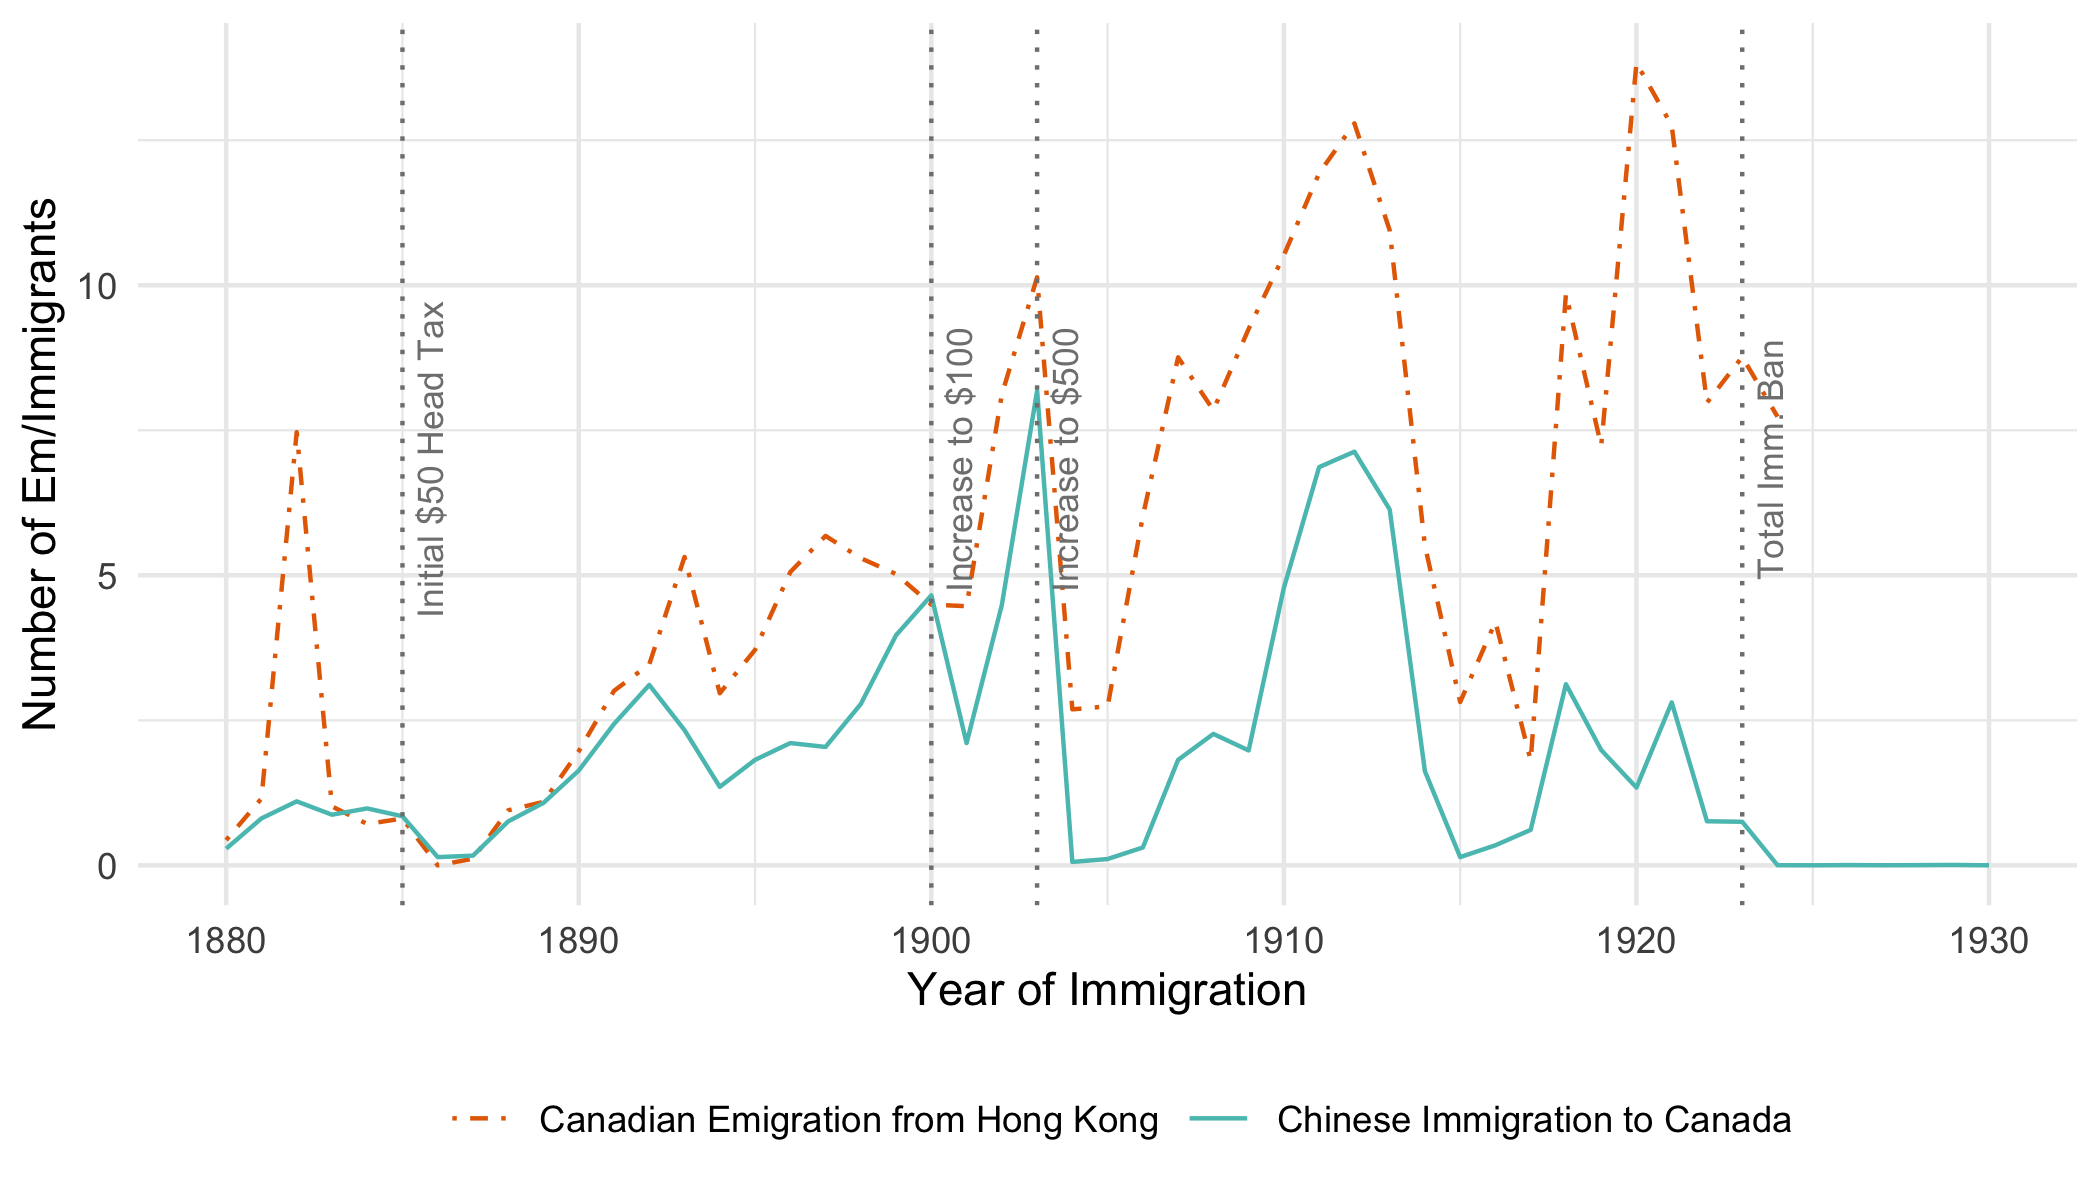
\includegraphics[width=\textwidth]{../../figs/fig2_flow_immandem.png}
    \label{fig:immandem}
\end{figure}
Appendix Figure \ref{fig:immandem} compares the number of Chinese emigrants from Hong Kong to Canada as reported in the Harbourmaster reports to the number of Chinese immigrants to Canada as reported in the Chinese Register from 1886 to 1923. In the first several years of the Head Tax, reported emigration aligns almost perfectly with reported immigration, but beginning in 1893, reported emigration consistently exceeds reported immigration, in some years by more than 5,000 migrants. 
This discrepancy can be explained in three ways. 
The first is that Chinese immigrants to Canada were permitted to leave and re-enter the country within a year without re-paying the Head Tax (or being re-recorded in the Register) upon re-entry. As a result, a returning Chinese immigrant who had already paid the Head Tax would be counted in the emigration data as a passenger on an emigrant ship to Canada, but would not be counted in the Register data as a new immigrant. 
The second is that beginning in 1887, migrants who were passing through Canada en route to another country were exempted from paying the tax, and also would not have been recorded in the Register.\footnote{Although it is possible that some Chinese emigrants were turned away because they could not afford to pay the Head Tax, historian Arlene Chan has told me that Chinese immigrants were generally aware of the tax prior to coming to Canada, indicating that deportation is unlikely to explain much of the discrepancy between emigration and immigration.}
Finally, it is unclear whether the emigration data include only Chinese passengers. If they include non-Chinese passengers, such as British citizens travelling between parts of the Commonwealth, then the discrepancy between emigration and immigration may be in part due to non-Chinese passengers, who would not be recorded as immigrants in the Chinese Register.

\newpage 

\section{The Effects of the Head Tax on the Immigrant Inflow of Other Countries}

I repeat the analysis from section 4 for all countries with at least 20 years of non-zero immigration flow to Canada in the Census between 1880 and 1920. To make coefficients comparable across countries, I use as my outcome variable the logarithm of the \textbf{migration rate}, i.e. the immigration flow divided by the origin country population. Normalizing by population also partially accounts for a lack of emigration data. I estimate the following equation:

\begin{multline}
    \label{eq:immflow3}
    \log(FLOW_{ct}/POP_{ct}) = \alpha_0 + \alpha_2 CANIMMIG_t + \alpha_3 POPSTOCK_{c, t-1} \\ + \alpha_4 (POPSTOCK_{c, t-1})^2 + \sum_{\tau \in \mathcal{T}^d} \gamma^c_\tau \mathbbm{1}[TAX_t = \tau]
\end{multline}

where $c$ indexes origin country and $POP_{ct}$ represents the population of country $c$ in year $t$.\footnote{I use decennial population estimates from \citet{maddison2010} and interpolate non-decennial years using a linear cubic spline.}

I graph $\gamma^c_{\tau}$ for all countries in Figure \ref{fig:gammac}. First, note that normalizing by population rather than controlling for emigration results in significantly negative coefficients in all Head Tax years for Chinese immigration, although $\gamma_{500}^c$ is the largest in magnitude, representing a roughly 200\% decrease in Chinese immigration flow associated with the \$500 Head Tax. In comparison, no other country has a significantly negative $\gamma_{\tau}$ in any year, with the exception of the UK for the \$50 Head Tax and Germany for the \$500 Head Tax. In summary, I find no significant and consistent effects of the Head Tax on immigration from any country other than China.

\begin{figure}[h!]
    \centering 
    \caption{Coefficients on Head Tax indicators in equation \ref{eq:immflow3} for countries all countries with both population data and at least 20 years of non-zero immigration flow to Canada in the Census between 1880 and 1920 \citep{census1901, census1911, census1921, maddison2010}.}
    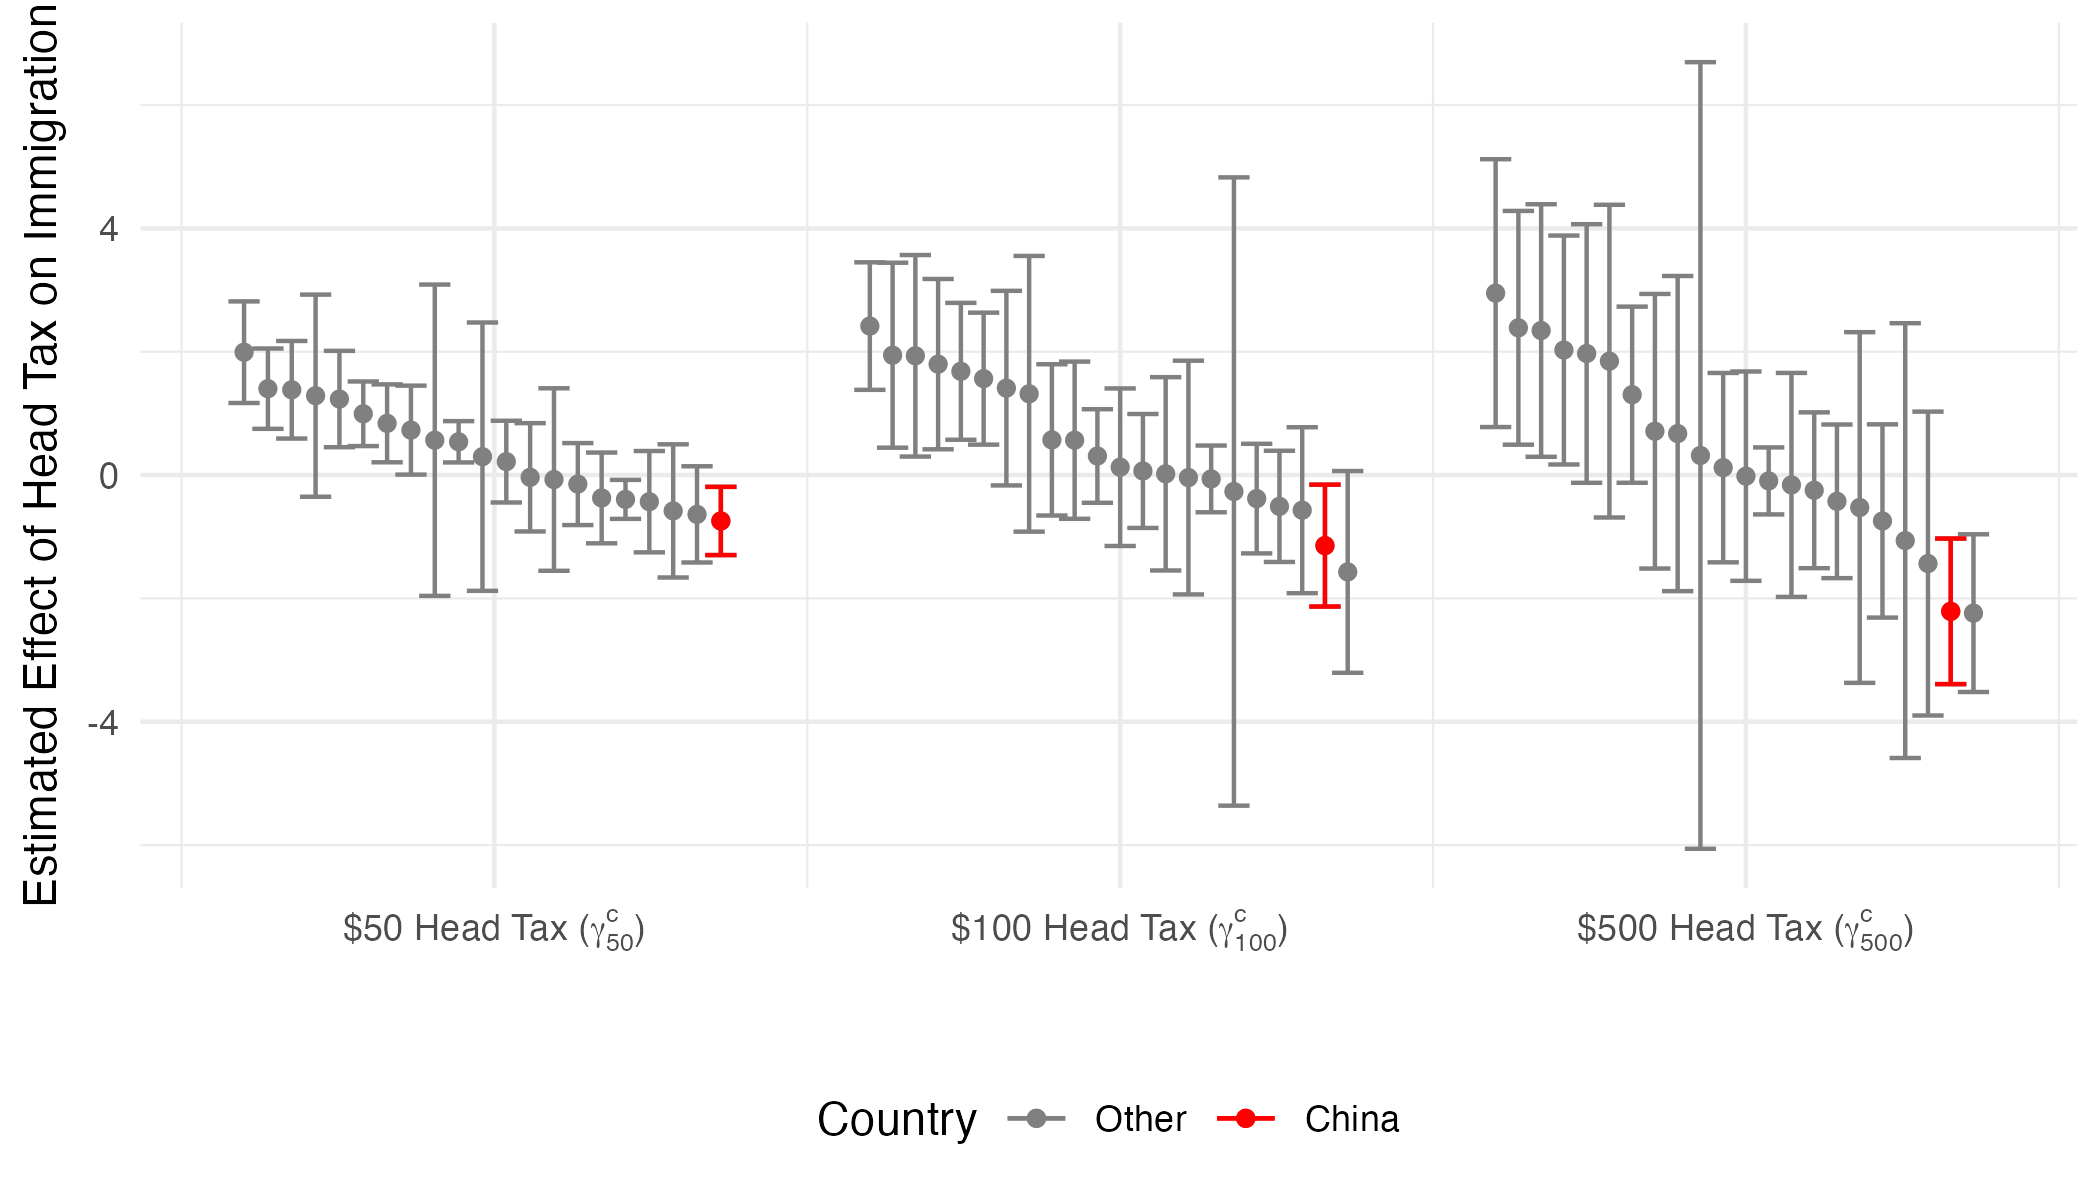
\includegraphics[width=\textwidth]{../../figs/immflow_countries.png}
    \label{fig:gammac}
\end{figure}
